\chapter{Research (HIGHT)}

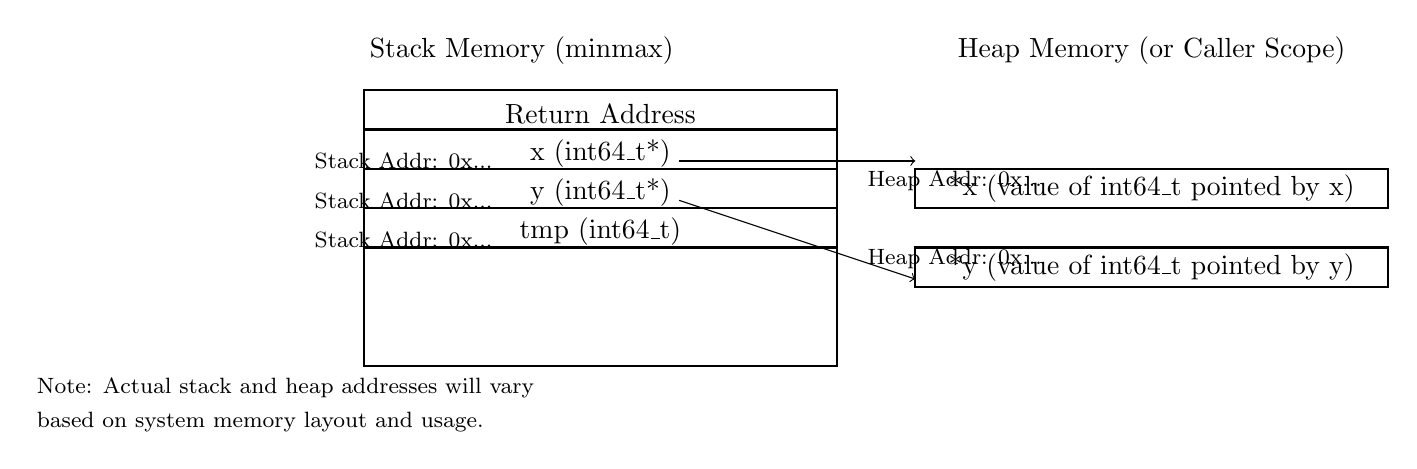
\begin{tikzpicture}
	% Title Labels
	\node at (-2,4) {Stack Memory (minmax)};
	\node at (6,4) {Heap Memory (or Caller Scope)};
	
	% Stack Frame for minmax function
	\draw[thick] (-4, 3.5) rectangle (2, 0);
	
	% Stack Frame Contents
	% Return Address
	\node at (-1, 3.2) {Return Address};
	\draw[thick] (-4, 3.0) -- (2, 3.0);
	
	% x parameter
	\node at (-1, 2.7) {x (int64\_t*)};
	\draw[thick] (-4, 2.5) -- (2, 2.5);
	\node at (-3.5, 2.6) {\footnotesize Stack Addr: 0x...};
	\draw[->] (0, 2.6) -- (3, 2.6); % Pointer arrow to heap x
	
	% y parameter
	\node at (-1, 2.2) {y (int64\_t*)};
	\draw[thick] (-4, 2.0) -- (2, 2.0);
	\node at (-3.5, 2.1) {\footnotesize Stack Addr: 0x...};
	\draw[->] (0, 2.1) -- (3, 1.1); % Pointer arrow to heap y
	
	% tmp local variable
	\node at (-1, 1.7) {tmp (int64\_t)};
	\draw[thick] (-4, 1.5) -- (2, 1.5);
	\node at (-3.5, 1.6) {\footnotesize Stack Addr: 0x...};
	
	% Heap Memory Visualization
	% Memory block for *x
	\draw[thick] (3, 2.5) rectangle (9, 2.0);
	\node at (6, 2.25) {*x (value of int64\_t pointed by x)};
	\node at (3.5, 2.35) {\footnotesize Heap Addr: 0x...};
	
	% Memory block for *y
	\draw[thick] (3, 1.5) rectangle (9, 1.0);
	\node at (6, 1.25) {*y (value of int64\_t pointed by y)};
	\node at (3.5, 1.35) {\footnotesize Heap Addr: 0x...};
	
	% Additional Notes
	\node at (-5, -0.5) [align=left] {\footnotesize Note: Actual stack and heap addresses will vary\\
		\footnotesize based on system memory layout and usage.};
	
\end{tikzpicture}